\documentclass[12pt,a4paper,]{scrreprt}
\usepackage[ngerman]{babel}
\usepackage[onehalfspacing]{setspace}
\usepackage[utf8]{inputenc}

\usepackage{graphicx,array,gnuplottex,siunitx,multicol,capt-of,amsmath,ulem,amsthm}
\let\phi\varphi
\setkomafont{chapter}{\fontsize{20bp}{22.2bp}\selectfont\bfseries}
\setkomafont{section}{\fontsize{12bp}{14.4bp}\selectfont\bfseries}

\renewcommand{\chapterheadstartvskip}{\vspace*{-1\topskip}}
\renewcommand{\chapterheadendvskip}{\vspace*{0.8\topskip}}
%---------------------------------------------------------------------------------------------------------------------------------------------------------------
% Ende der Einstellungen
%---------------------------------------------------------------------------------------------------------------------------------------------------------------

%---------------------------------------------------------------------------------------------------------------------------------------------------------------
%Ab hier gibt es Inhalt
%---------------------------------------------------------------------------------------------------------------------------------------------------------------
\begin{document}

\title{Gekoppelte Pendel}
\author{Henrik Jäger \\ 3114168 \and Lena Majer \\ 3115808}
\subtitle{M23a \\  Assistentin: Ramona Tschüter}
\subject{Physikalisches Praktikum I}
\publishers{Universität Stuttgart}
\date{26. Januar 2017}
%\thanks{Assistent: Sascha Kolatschek}

\maketitle% Titelei

\tableofcontents   %Inhaltsverzeichnis
\pagebreak
\chapter{Einleitung}
\section{Ziel}
Das Ziel dieses Versuches ist die Bestimmung des Kopplungsgrades zweier Pendel. Hierfür werden die Periodendauern verschiedener Schwinungsarten der gekoppelten Pendel bestimmt.
\section{Grundlagen}
Unter einem mathematischen Pendel versteht man ein Pendel, das aus einem Massenlosen Stab und einer Punktmasse besteht.
Unter einem physikalischen Pendel versteht man einen langen starren Stab, der am Ende aufgehängt ist.
Im Folgenden Versuch werden zwei mathematisches Pendel, ohne Raumausdehnung,  betrachtet. Diese Pendel sind miteinander gekoppelt. Bei diesem Pendel muss somit die potentielle Energie der Feder und die Gravitation  berücksichtigt werden.
%Die Lagrangefunktion ist gegeben durch:\\
%\begin{equation}
%L= 1/2 I \dot{\Psi_1}+ 1/2 I \dot{\Psi_2} + m*g*L*cos(\Psi_1) + m*g*L*cos(\Psi_2) - 1/2D_F*l^2(sin(\Psi_1) – sin(\Psi_2))^2\\
%\end{equation}

%L = kinetische Energie – Gravitationspotential – Federpotential\\
Über Euler-Lagrange können die Bewegungsgleichungen aufgestellt werden. Diese sind gegeben durch:
\begin{equation}
I\frac{d^2\Psi _1}{dt^2}= -m\cdot g\cdot L\cdot\Psi_1 – D\cdot l^2(\Psi_1 - \Psi_2)
\end{equation}
\begin{equation}
I\frac{d^2\Psi _2}{dt^2}= - m\cdot g\cdot L\cdot\Psi_1 – D\cdot l^2(\Psi_2 - \Psi_2)
\end{equation}
I steht für das Trägheitsmoment, m entspricht der Masse des Pendelkörpers, D ist die Federkonstante, $\Psi$ steht für die verschiedenen Auslenkungswinkeln, L entspricht der Länge des Pendels und l beschreibt den Abstand zwischen der Feder und der Aufhängung. Nach Lösen der Bewegungsgleichung erhält man zwei Fundamentallösungen, die für zwei Fundamentalschwingungen stehen. \
 Diese Fundamentalschwingungen beschreiben  die Schwingung der beiden Pendelkörper miteinander – ohne Phasenverschiebung. Dies nennt man auch symmetrische Schwingung. \ 
 Die zweite Fundamentalschwingung hat eine Phasenverschiebung der Größe  $\pi$.  Alle weiteren Lösungen sind durch Linearkombinationen der beiden Fundamentalschwingungen gefunden. Dies wird auch antisymmetrische Schwingung genannt. Unter dem Schwebungsfall versteht man eine Superposition aus den beiden Fundamentalschwingungen.% Als Lösung der Differentialgleichung  erhält man hierfür: \\
%\begin{equation}
%\Psi_1 (t) = \Psi_a * cos (w_(II)*t) 
%\end{equation}
%\begin{equation}
%\Psi_2 (t) = \Psi_a * cos (w_(II)*t) 
%\end{equation}



\chapter{Messprinzip mit Skizze und Versuchsablauf}
In diesem Versuch sind zwei physikalische Pendel gegeben. Zunächst wird die Schwingdauer der Pendel ohne Kopplung bestimmt. Anschließend wird eine Kopplung zwischen den zwei Pendeln in einer Höhe von $20\si{\centi\metre}$ montiert. Daraufhin wird die gleichphasige Schwingung und gegenläufige Schwingung über zehn Perioden bestimmt.
Zuletzte wird die Schwebungsdauer und die hierbei verbundene Periodendauer der Pendel bestimmt.
Dies wird für drei weitere Kopplungsgrade ($35\si{\centi\metre}$, $50\si{\centi\metre}$,$65\si{\centi\metre}$) wiederholt.
\begin{center}

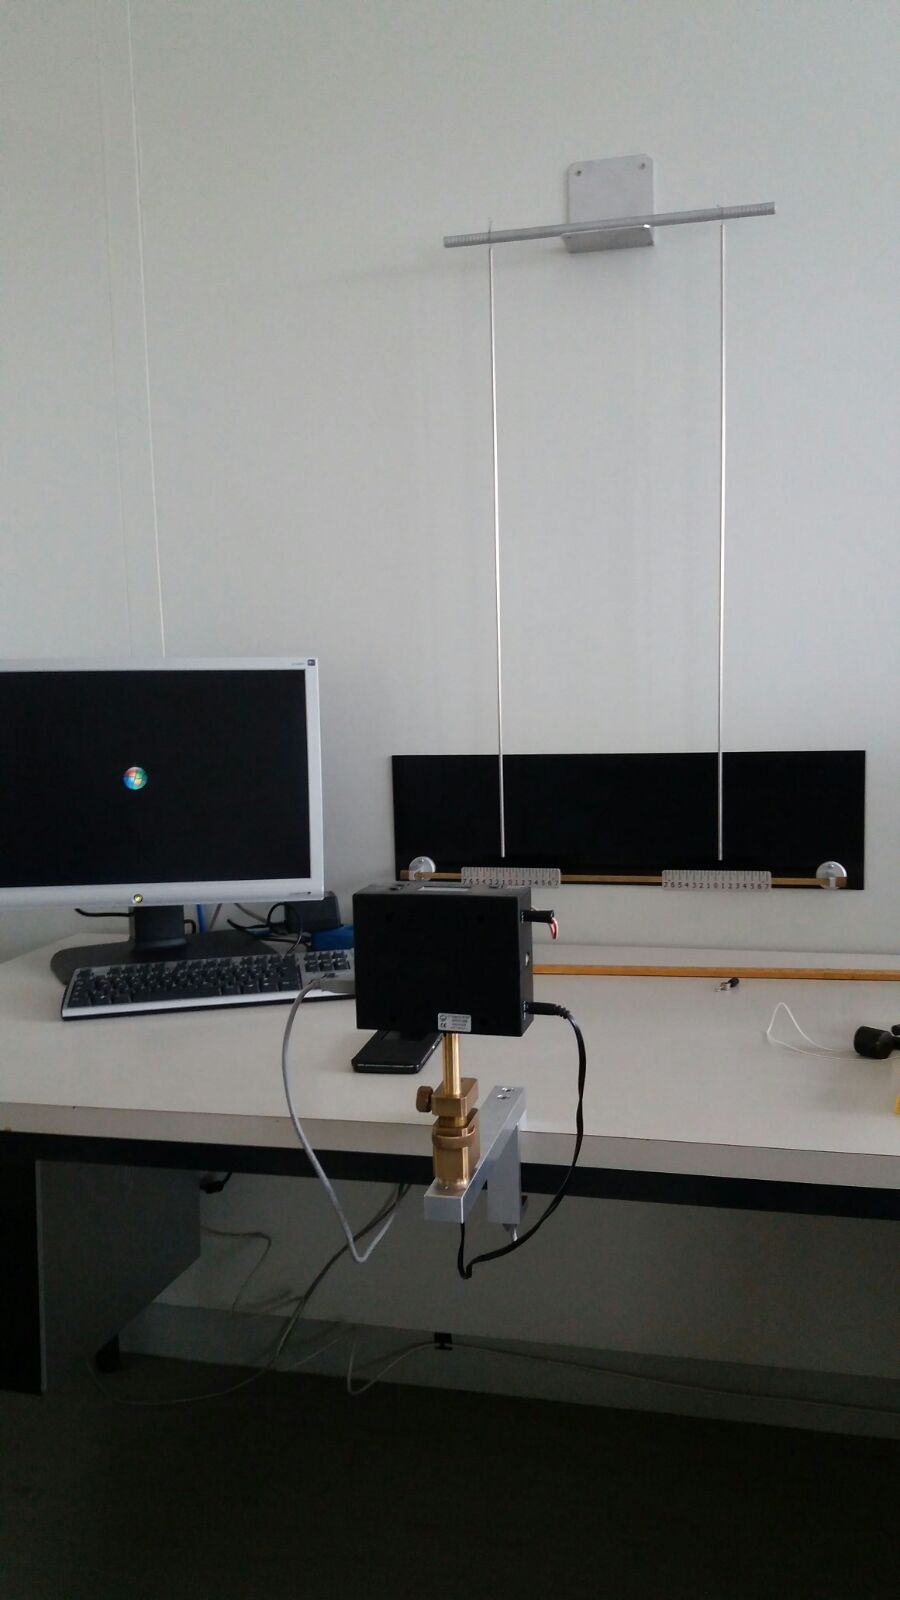
\includegraphics[scale=0.25]{2.jpg}
\captionof{figure}[]{Versuchsaufbau}
\end{center}


	\chapter{Formeln}
    Den Kopplungsgrad K der gekoppelten Pendeln bestimmt man über die verschiedenen Schwingdauern T. Hierfür gilt:
    \begin{equation}
    K_1=\frac{T^2_{gl}-T^2_{geg}}{T^2_{gl}+T^2_{geg}}
    \end{equation}
    \begin{equation}
    K_2=4 \cdot \frac{T_S T_{II}}{4T^2_{S}+T^2_{II}}
    \end{equation}
	\pagebreak



	\chapter{Messwerte}
  \begin{center}
  
    \begin{tabular}{c||c|c|c|c}
    $l~[cm] $& $10T_{gl}~[s]$ & $10T_{gg}~[s]$ &	$5T_{s}~[s]$ & $10T_{II}~[s]$ \\ \hline \hline
		&17,2	&17,1	&514,6 (4 Perioden)	&17,1\\
	20	&17,2	&17,05	&647	&17,1\\
		&17,3	&17		&640,9	&17,1\\ \hline
		&17,05	&16,6	&223,7	&17,1\\
	35	&17,1	&16,5	&221,7	&16,9\\
		&17,2	&16,6	&222	&16,9\\ \hline
		&17,2	&16,1	&118,1	&16,6\\
	50	&17,12	&16		&119	&16,5\\
		&17,2	&16		&117,2	&16,6\\ \hline
		&17,2	&15,5	&75,4	&17,2\\
	65	&17,3	&15,5	&76,2	&17,1\\
		&17,2	&15,4	&76,3	&17,1\\
    \end{tabular}
    \captionof{table}[]{Messwerte}
  \end{center}
     $10T_0=17,2s$
	\pagebreak

	\chapter{Auswertung}
    	\section{Germanium- und Siliziumdioden in Durchlassrichtung}
        	\begin{gnuplot}[terminal=pdf,terminaloptions={font ",10" linewidth 2},scale=1.2]
            		set fit errorvariables
					
                  	set xlabel "Spannung [V]"
                  	set ylabel "Stromstärke [mA]"
					set xrange [0:1]
                    set yrange [0:1]
                    
                    f(x) = a*exp(b*x)
                    g(x) = c*exp(d*x)
                    fit f(x) "Daten/A1a.txt" using 2:1 via a,b
                    fit g(x) "Daten/A1a.txt" using 3:1 via c,d
                    
                  	plot "Daten/A1a.txt" using 2:1 title "Germanium", "Daten/A1a.txt" using 3:1 title "Silizium", f(x), g(x)
			\end{gnuplot}
        \captionof{figure}[DurchlassGerSil]{Kennlinien der Dioden in Durchlassrichtung}
        Im Diagramm wurde die Fitfunktion 			
        \begin{equation}
        	f(x) = a \cdot \exp(b\cdot x)
        \end{equation}
        verwendet. \\
        
        Wenn wir davon ausgehen, dass Formel \ref{Sperrstrom-vereinfacht} gilt, können wir den Sperrstrom aus den gefitteten Werten ermitteln. \\
        
        Es ergibt sich:
	\begin{center}
		\begin{tabular}{c|cc}
			&  Germanium & Silizium\\ \hline
    		$I_s$ & $0.3\cdot 10^{-3} mA$ &  $0.04\cdot 10^{-6} mA$
		\end{tabular}
    \end{center}    
   		     
        
        \pagebreak
        
        \section{Germanium- und Silizium in Sperrrichtung}
        \begin{gnuplot}[terminal=pdf,terminaloptions={font ",10" linewidth 2},scale=1.2]
        	set xlabel "Spannung [V]"
			set ylabel "Stromstärke [Mikroampere]"
            
			f(x)=a*x+b
            g(x)=c*x+d
            
            set key left
            
            set xrange [-8:0]
            
            fit f(x) "Daten/A1c.txt" using 1:2 via a,b
            fit g(x) "Daten/A1c.txt" using 1:3 via c,d
           	
            plot "Daten/A1c.txt" using 1:2 title "Germanium", "Daten/A1c.txt" using 1:3 title "Silizium", f(x), g(x)
                    
			\end{gnuplot}
        \captionof{figure}[DurchlassGerSil]{Kennlinien der Dioden in Sperrrichtung}
        
       \ \\
       Die Werte passen nicht zu den im ersten Versuchsteil bestimmten Sperrströmen
        \pagebreak
        
        \section{Zenerdiode in Durchlass- und Sperrrichtung}
        	Trägt man Durchlass und Sperrrichtungskennlinien in einem gemeinsamen Diagramm auf erhält man die Z-Linie. \\
        	\begin{gnuplot}[terminal=pdf,terminaloptions={font ",10" linewidth 2},scale=1.2]
					
                  	set xlabel "Spannung [V]"
                  	set ylabel "Stromstärke [Mikroampere]"
                  	
                  	plot "Daten/A2a.txt" using 2:1 title "Durchlassrichtung", "Daten/A2b.txt" using 1:2 title "Sperrrichtung 
			\end{gnuplot}
        \captionof{figure}[DurchlassGerSil]{Gesamtkennlinie der Zener-Diode} 
        \ \\
        Hier spielt in der Sperrrichtung die spezielle Eigenschaft der Zener-Diode eine Rolle. Ab einer gewissen Sperrspannung nimmt ihr differentieller Widerstand exponentiell zu, während er vor dieser Spannung noch nicht vorhanden war.\ \\
        Bei einer Spannung von $ U = 5,75 V$ wurde mit der $\mu A$ -Skala ein Strom von $948 \mu A$ gemessen. Mit der mA-Skala wurde aber ein Strom von $960 \mu A$ gemessen. Die $\mu A$-Skala ist auf genaueres Messen ausgelegt, während die mA-Skala höhere Ströme aushält.
        
        \pagebreak
        
        \section{LEDs mit Oszilloskop}
        \begin{center}
        
         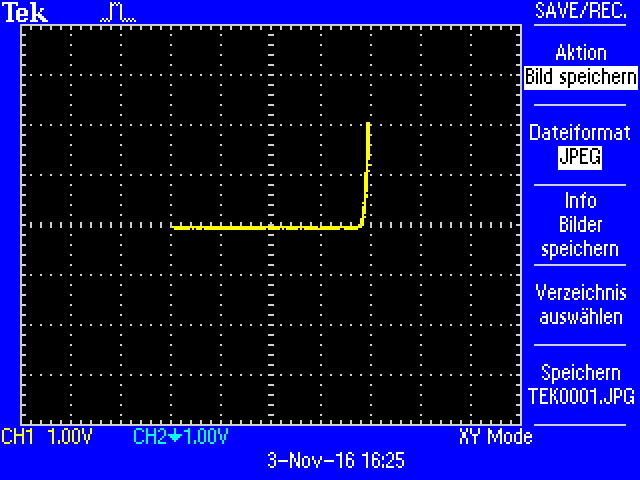
\includegraphics[scale=1]{Daten/TEK0001.JPG}
           \captionof{figure}[DurchlassGerSil]{Kennlinie der roten LED} 
         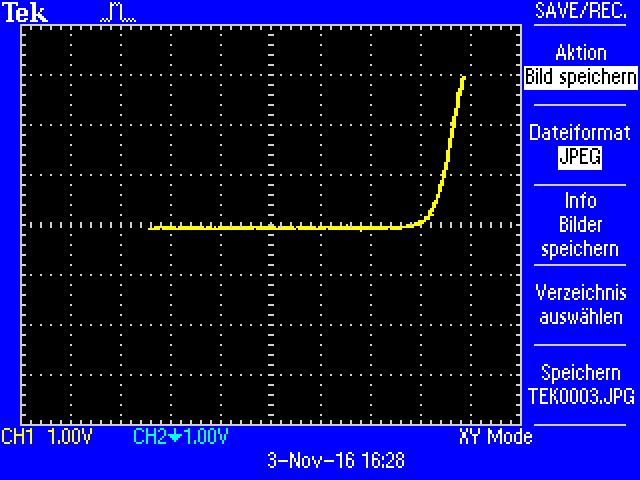
\includegraphics[scale=1]{Daten/TEK0003.JPG}
           \captionof{figure}[DurchlassGerSil]{Kennlinie der blauen LED} 
           \end{center}
        
       Die Schwellspannungen sind aus den Diagrammen abzulesen und sind:
       \begin{center}
       \begin{tabular}{c|c}
       &Schwellspannung\\ \hline
       Rot & $1,8 V$ \\
       Blau & $2,7 V$
       \end{tabular}
       \end{center}
       Damit lässt sich die Wellenlänge des Lichtes berechnen, das von der LED abgestrahlt wird.
       \begin{align*}
       		\lambda_{rot} & = \frac{h \cdot c}{e \cdot U_{rot}} \\
            & = \frac{6,626 \cdot 10^{-34} Js \cdot 0,3 \cdot 10^9 \frac{m}{s}}{1,6 \cdot 10^{-19} C \cdot 1,8 V} = 690,2 nm
       \end{align*} 
       \begin{align*}
       		\lambda_{blau} & = \frac{h \cdot c}{e \cdot U_{blau}} \\
            & = \frac{6,626 \cdot 10^{-34} Js \cdot 0,3 \cdot 10^9 \frac{m}{s}}{1,6 \cdot 10^{-19} C \cdot 2,7 V} = 460,1 nm
       \end{align*}
       
       Die errechneten Wellenlängen passen sehr gut zum Licht, dass von den LEDs abgestrahlt wird, wenn man für blaues Licht eine Wellenlänge von $420nm$ bis $490nm$ und $650nm$ bis $750nm$ für rotes Licht annimmt. \footnote{https://de.wikipedia.org/wiki/Licht}
	\pagebreak


	\chapter{Fehlerrechnung}
	Um das Ventilvolumen in die Formel einzubringen, wird $\gamma$ in Abhängigkeit der Länge $l$, statt der Fläche $A$ und dem Volumen $V$ geschrieben.
      \begin{align*}
     		\gamma = \frac{16 \pi \cdot m \cdot l \cdot f_0^2}{d^2 \cdot p_0}
      \end{align*}
      \begin{align*}
     		\Delta\gamma_{\text{Luft}} &= 
            \left| \frac{16\pi l f_0^2}{d^2 p_0}\right| \Delta m + 
            \left| \frac{16\pi m f_0^2}{d^2 p_0}\right| \Delta l + 
            \left| \frac{32\pi m l f_0}{d^2 p_0}\right| \Delta f_0 + 
            \left| -\frac{32 \pi m l f_0^2}{d^3 p_0}\right| \Delta d \\&+ 
            \left| -\frac{16 \pi m l f_0^2}{d^2 p_0^2}\right| \Delta p_0 \\&=
            \left| \frac{16\pi (0,45m + 0,001m) (13,4Hz)^2}{(0,016m)^2 (103100Pa)}\right| (0,0000001kg)\\ &+ 
            \left| \frac{16\pi (0,0088781kg) (13,4Hz)^2}{(0,016m)^2 (103100Pa)}\right| (0,001m) \\ &+ 
            \left| \frac{32\pi (0,0088781kg) (0,45m + 0,001m) (13,4Hz)}{(0,016m)^2 (103100Pa)}\right| (0,2Hz) \\ &+ 
            \left| -\frac{32 \pi (0,0088781kg) (0,45m + 0,001m) (13,4Hz)^2}{(0,016m)^3 (103100Pa)}\right| (0,00001m)\\&+ 
            \left| -\frac{16 \pi (0,0088781kg) (0,45m + 0,001m) (13,4Hz)^2}{(0,016m)^2 (103100Pa)^2}\right| (100Pa) \\ &= 0,048
      \end{align*} \\
      
      Analog für die weiteren Fehler
      \begin{center}
      \begin{tabular}{c|c}
$l ~[\text{m}]$ & $\Delta\gamma ~[1]$    \\ \hline
0,45         & 0,048 \\
0,40          & 0,045\\
0,35         & 0,045 \\
0,30          & 0,042 \\
0,25         & 0,039 \\
0,20          & 0,037 \\
0,15         & 0,036 \\
0,10          & 0,035	
		\end{tabular}
	\end{center}
      
\captionof{table}[]{Fehler für die Messung mit Luft als Kolbenfüllung.}
\begin{center}
      \begin{tabular}{c|c}
$l ~[\text{m}]$ & $\Delta\gamma ~[1]$    \\ \hline
0,45 & 0,048 \\
0,40  & 0,045 \\
0,35 & 0,042 \\
0,30  & 0,040 \\
0,25 & 0,038 \\
0,20  & 0,036 \\
0,15 & 0,035 \\
0,10  & 0,034
		\end{tabular}
	\end{center}
      
\captionof{table}[]{Fehler für die Messung mit Kohlenstoffdioxid als Kolbenfüllung.}

\begin{center}
      \begin{tabular}{c|c}
$l ~ [\text{m}]$ & $\Delta\gamma ~[1]$    \\ \hline
0,45   & 0,053 \\
0,40    & 0,050 \\
0,35   & 0,048 \\
0,30    & 0,045 \\
0,24   & 0,042 \\
0,19   & 0,038 \\
0,14   & 0,047 \\
0,095  & 0,038 
		\end{tabular}
	\end{center}
      
\captionof{table}[]{Fehler für die Messung mit Argon als Kolbenfüllung.}
\ \\
Es soll nur ein Wert für den Fehler angegeben werden. Anstatt wie bei den Messwerten zu mitteln, wird hier jedoch der größte Fehler angenommen, damit der Fehlerwert nicht zu gering ausfällt.

\begin{align*}
 	\Delta \gamma_{\text{Luft}} & = 0,048\\
    \Delta \gamma_{\text{CO}_2} & = 0,048\\
    \Delta \gamma_{\text{Argon}}& = 0,053
\end{align*}

     	\section{Mögliche Abweichungen}
        	Im Versuch wird angenommen, dass die Erregerfrequenz beim Maximum der Schwingung der Eigenfrequenz des ungedämpften Systems entspricht. Durch Dämpfung fällt die Frequenz jedoch geringer aus, was sich durch den Zusammenhang $\gamma \propto f^2$ stark auf das Ergebnis auswirkt. Der Wert für den gemessenen Adiabatenexponent liegt also unter dem tatsächlichen. Außerdem wird nicht mit einem isolierten System gemessen, sodass der Vorgang nicht vollständig adiabatisch verläuft. Reibung verursacht ebenfalls einen Fehler.
	\pagebreak

	\chapter{Zusammenfassung}
    In diesem Versuch wurden die Schwingdauern von gekoppelten Pendel gemessen. Aus diesen Schwingdauern wurden die Kopplungen bestimmt.\\
    \\
    Für die Kopplungen erhielt man die Werte:
    \begin{center}
    \begin{tabular}{c||c|c}
     $l~[cm] $& $\Delta K_1~[1]$ & $\Delta K_2~[1]$ \\ \hline \hline
	20&$0,0107\pm 0,0580$&$0,0133\pm0,0004$\\
	35&$0,0326\pm 0,0584$&$0,0381\pm0,0010$\\
	50&$0,0686\pm 0,0580$&$0,0701\pm0,0018$\\
	65&$0,1077\pm 0,0574$&$0,1124\pm0,0025$\\
   \end{tabular}
   \captionof{table}[]{Endergebnis}
    \end{center}
   
Fehlerquellen waren Ungenauigkeiten der Messaperaturen. Zudem ist es nur sehr schwer möglich eine reine gleichphasige oder gegenphasige Schwingung zu erzeugen.

	\chapter{Anhang}
    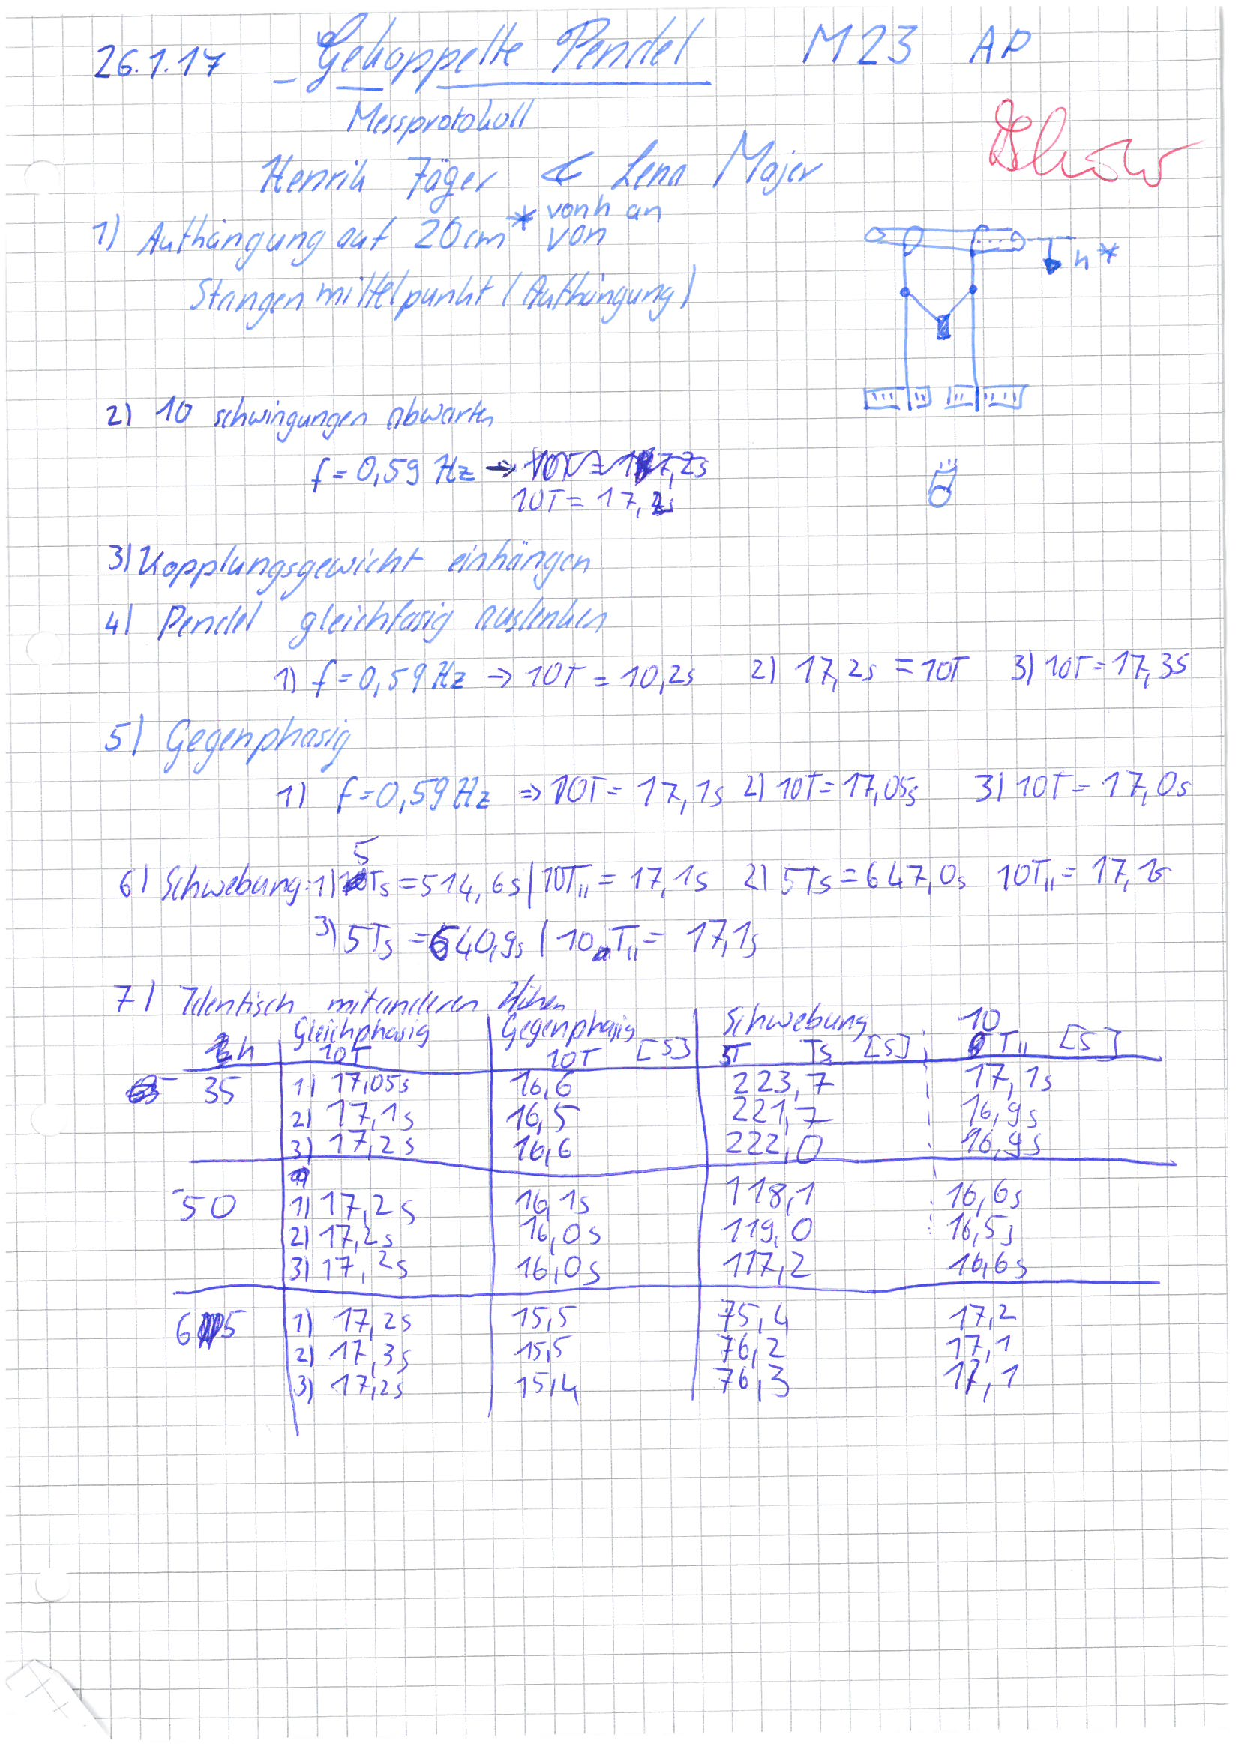
\includegraphics[scale=0.75]{1.pdf}
	\pagebreak











\end{document}
